\documentclass[docid=TP06]{tcom_TP}
\begin{document}
\setcounter{section}{5}
\section{TP06 - Regular languages}
{
\renewcommand{\thesubsubsection}{\thesubsection\alph{subsubsection}}
\subsection{Exercise 1}
\subsubsection{Item a}
\begin{center} 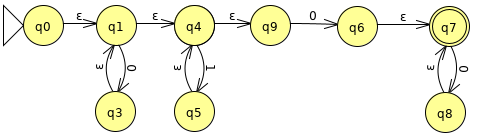
\includegraphics[scale=0.5]{TP06_1_a} \end{center}
\subsubsection{Item b}
\begin{center} 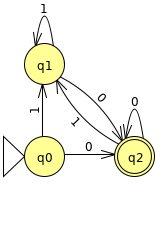
\includegraphics[scale=0.5]{TP06_1_b} \end{center}
\subsubsection{Item c}
\begin{center} 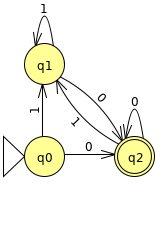
\includegraphics[scale=0.5]{TP06_1_b} \end{center}
\subsubsection{Item d}
\begin{center} 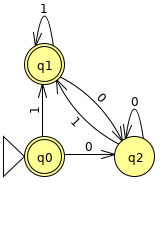
\includegraphics[scale=0.5]{TP06_1_d} \end{center}
\subsection{Exercise 2}
\subsubsection{Item a}
\begin{alignat*}{2}
	NFA N    &= (Q_N, \Sigma, \delta_N, q_0, F_N)\\
	Q_N      &= \{1,2,3,4\}\\
	\Sigma   &= \{a,b\}\\
	q_0      &= 1\\
	F_N      &= \{2\}\\
	\delta_N &\colon Q_N \times \Sigma \rightarrow \mathscr{P}(Q_N)
\end{alignat*}
\subsubsection{Item b}
\begin{center} \begin{tabular}{r | c c}
	$\delta_N     $ & $a      $ & $b    $ \\ \hline
	$\rightarrow 1$ & $\{1,2\}$ & $\{3\}$ \\
	$      ^* 2$ & $\emptyset$ & $\{1\}$ \\
	$            3$ & $\{4\}  $ & $\{2\}$ \\
	$            4$ & $\{2,3\}$ & $\{4\}$
\end{tabular} \end{center}
\subsubsection{Item c}
\begin{center} \begin{tabular}{r | c c}
	$\delta_N     $ & $a      $ & $b    $ \\ \hline
	$\rightarrow \{1    \}$ & $\{1,2  \}$ & $\{3    \}$\\
	$      ^* \{2    \}$ & $\emptyset$ & $\{1    \}$\\
	$            \{3    \}$ & $\{4    \}$ & $\{2    \}$\\
	$            \{4    \}$ & $\{2,3  \}$ & $\{4    \}$\\
	$      ^* \{1,2  \}$ & $\{1,2  \}$ & $\{1,3  \}$\\
	$            \{1,3  \}$ & $\{1,2,4\}$ & $\{2,3  \}$\\
	$      ^* \{2,3  \}$ & $\{4    \}$ & $\{1,2  \}$\\
	$      ^* \{1,2,3\}$ & $\{1,2,4\}$ & $\{1,2,3\}$\\
	$      ^* \{1,2,4\}$ & $\{1,2,3\}$ & $\{1,3,4\}$\\
	$            \{1,3,4\}$ & $\{1,2,3,4\}$ & $\{2,3,4\}$\\
	$      ^* \{2,3,4\}$ & $\{2,3,4\}$ & $\{1,2,4\}$\\
	$      ^* \{1,2,3,4\}$ & $\{1,2,3,4\}$ & $\{1,2,3,4\}$
\end{tabular} \end{center}
\begin{center} 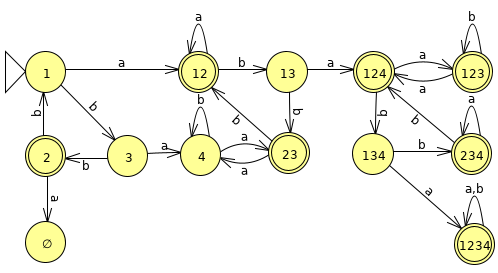
\includegraphics[scale=0.5]{TP06_2_d} \end{center}
\subsection{Exercise 3}
\begin{equation*}
	b^* a b^* a (a+b)^*
\end{equation*}
\subsection{Exercise 4}
\begin{alignat*}{2}
	     & L(b^*a^*)\cap L(a^*b^*) = L(a^*) \cup L(b^*)\\
	\iff & (L(\varepsilon) \cup L(a^+) \cup L(b^+) \cup L(b^+a^+))\cap (L(\varepsilon) \cup L(a^+) \cup L(b^+) \cup L(a^+b^+)) = L(a^*) \cup L(b^*)\\
	\iff & L(\varepsilon) \cup L(a^+) \cup L(b^+) = L(a^*) \cup L(b^*)\\
	\iff & L(\varepsilon) \cup L(a^+) \cup L(b^+) = (L(\varepsilon)\cup L(a^+)) \cup (L(\varepsilon)\cup L(b^+))\\
	\iff & L(\varepsilon) \cup L(a^+) \cup L(b^+) = L(\varepsilon)\cup L(a^+) \cup L(b^+)
\end{alignat*}
We have thus proven this equality correct.
\subsection{Exercise 5}
\begin{center} \begin{tabular}{r | c c}
	$\delta_D       $ & $0  $ & $1  $ \\ \hline
	$\rightarrow q_1$ & $q_2$ & $q_3$\\
	$            q_2$ & $q_1$ & $q_3$\\
	$         ^* q_3$ & $q_2$ & $q_1$
\end{tabular} \end{center}
Aside from accept states, this DFA is the same as the one presented in TP05.10 and what is asked is a part of the solution of TP05.10a. I thus advise you to see the solution for TP05.10, which contains all middle steps requested in this exercise and leads to the following answer:
\begin{equation*}
	R_{13}^{(3)} = 0^*1((0+1)0^*1)^*
\end{equation*}
\subsection{Exercise 6}
\subsubsection{Item a}
False, given the DFA equivalent to an NFA with $k$ states can have up to or exactly $2^k$ states.
\subsubsection{Item b}
True, given that $L^0 \subseteq L^*$ and $L^0=\{\varepsilon\}$.
}
\end{document}
